\documentclass[twoside]{book}

% Packages required by doxygen
\usepackage{fixltx2e}
\usepackage{calc}
\usepackage{doxygen}
\usepackage[export]{adjustbox} % also loads graphicx
\usepackage{graphicx}
\usepackage[utf8]{inputenc}
\usepackage{makeidx}
\usepackage{multicol}
\usepackage{multirow}
\PassOptionsToPackage{warn}{textcomp}
\usepackage{textcomp}
\usepackage[nointegrals]{wasysym}
\usepackage[table]{xcolor}

% Font selection
\usepackage[T1]{fontenc}
\usepackage[scaled=.90]{helvet}
\usepackage{courier}
\usepackage{amssymb}
\usepackage{sectsty}
\renewcommand{\familydefault}{\sfdefault}
\allsectionsfont{%
  \fontseries{bc}\selectfont%
  \color{darkgray}%
}
\renewcommand{\DoxyLabelFont}{%
  \fontseries{bc}\selectfont%
  \color{darkgray}%
}
\newcommand{\+}{\discretionary{\mbox{\scriptsize$\hookleftarrow$}}{}{}}

% Page & text layout
\usepackage{geometry}
\geometry{%
  a4paper,%
  top=2.5cm,%
  bottom=2.5cm,%
  left=2.5cm,%
  right=2.5cm%
}
\tolerance=750
\hfuzz=15pt
\hbadness=750
\setlength{\emergencystretch}{15pt}
\setlength{\parindent}{0cm}
\setlength{\parskip}{3ex plus 2ex minus 2ex}
\makeatletter
\renewcommand{\paragraph}{%
  \@startsection{paragraph}{4}{0ex}{-1.0ex}{1.0ex}{%
    \normalfont\normalsize\bfseries\SS@parafont%
  }%
}
\renewcommand{\subparagraph}{%
  \@startsection{subparagraph}{5}{0ex}{-1.0ex}{1.0ex}{%
    \normalfont\normalsize\bfseries\SS@subparafont%
  }%
}
\makeatother

% Headers & footers
\usepackage{fancyhdr}
\pagestyle{fancyplain}
\fancyhead[LE]{\fancyplain{}{\bfseries\thepage}}
\fancyhead[CE]{\fancyplain{}{}}
\fancyhead[RE]{\fancyplain{}{\bfseries\leftmark}}
\fancyhead[LO]{\fancyplain{}{\bfseries\rightmark}}
\fancyhead[CO]{\fancyplain{}{}}
\fancyhead[RO]{\fancyplain{}{\bfseries\thepage}}
\fancyfoot[LE]{\fancyplain{}{}}
\fancyfoot[CE]{\fancyplain{}{}}
\fancyfoot[RE]{\fancyplain{}{\bfseries\scriptsize Generated by Doxygen }}
\fancyfoot[LO]{\fancyplain{}{\bfseries\scriptsize Generated by Doxygen }}
\fancyfoot[CO]{\fancyplain{}{}}
\fancyfoot[RO]{\fancyplain{}{}}
\renewcommand{\footrulewidth}{0.4pt}
\renewcommand{\chaptermark}[1]{%
  \markboth{#1}{}%
}
\renewcommand{\sectionmark}[1]{%
  \markright{\thesection\ #1}%
}

% Indices & bibliography
\usepackage{natbib}
\usepackage[titles]{tocloft}
\setcounter{tocdepth}{3}
\setcounter{secnumdepth}{5}
\makeindex

% Hyperlinks (required, but should be loaded last)
\usepackage{ifpdf}
\ifpdf
  \usepackage[pdftex,pagebackref=true]{hyperref}
\else
  \usepackage[ps2pdf,pagebackref=true]{hyperref}
\fi
\hypersetup{%
  colorlinks=true,%
  linkcolor=blue,%
  citecolor=blue,%
  unicode%
}

% Custom commands
\newcommand{\clearemptydoublepage}{%
  \newpage{\pagestyle{empty}\cleardoublepage}%
}

\usepackage{caption}
\captionsetup{labelsep=space,justification=centering,font={bf},singlelinecheck=off,skip=4pt,position=top}

%===== C O N T E N T S =====

\begin{document}

% Titlepage & ToC
\hypersetup{pageanchor=false,
             bookmarksnumbered=true,
             pdfencoding=unicode
            }
\pagenumbering{roman}
\begin{titlepage}
\vspace*{7cm}
\begin{center}%
{\Large Soft\+Maker }\\
\vspace*{1cm}
{\large Generated by Doxygen 1.8.11}\\
\end{center}
\end{titlepage}
\clearemptydoublepage
\tableofcontents
\clearemptydoublepage
\pagenumbering{arabic}
\hypersetup{pageanchor=true}

%--- Begin generated contents ---
\chapter{Hierarchical Index}
\section{Class Hierarchy}
This inheritance list is sorted roughly, but not completely, alphabetically\+:\begin{DoxyCompactList}
\item \contentsline{section}{softmakerjava.\+Code\+Editor}{\pageref{classsoftmakerjava_1_1_code_editor}}{}
\item \contentsline{section}{softmakerjava.\+Employee\+Panel}{\pageref{classsoftmakerjava_1_1_employee_panel}}{}
\item \contentsline{section}{softmakerjava.\+General\+Settings\+Editor}{\pageref{classsoftmakerjava_1_1_general_settings_editor}}{}
\item \contentsline{section}{softmakerjava.\+Info\+Center}{\pageref{classsoftmakerjava_1_1_info_center}}{}
\item J\+Frame\begin{DoxyCompactList}
\item \contentsline{section}{softmakerjava.\+Code\+Viewer}{\pageref{classsoftmakerjava_1_1_code_viewer}}{}
\item \contentsline{section}{softmakerjava.\+Login\+Form}{\pageref{classsoftmakerjava_1_1_login_form}}{}
\item \contentsline{section}{softmakerjava.\+Main\+Frame}{\pageref{classsoftmakerjava_1_1_main_frame}}{}
\item \contentsline{section}{softmakerjava.\+Server\+Acess\+Window}{\pageref{classsoftmakerjava_1_1_server_acess_window}}{}
\item \contentsline{section}{softmakerjava.\+Settings\+Panel}{\pageref{classsoftmakerjava_1_1_settings_panel}}{}
\end{DoxyCompactList}
\item \contentsline{section}{softmakerjava.\+Manager\+Center}{\pageref{classsoftmakerjava_1_1_manager_center}}{}
\item \contentsline{section}{softmakerjava.\+Server\+Handler}{\pageref{classsoftmakerjava_1_1_server_handler}}{}
\item \contentsline{section}{softmakerjava.\+Settings}{\pageref{classsoftmakerjava_1_1_settings}}{}
\item \contentsline{section}{softmakerjava.\+Soft\+Maker\+Java}{\pageref{classsoftmakerjava_1_1_soft_maker_java}}{}
\item \contentsline{section}{softmakerjava.\+Task}{\pageref{classsoftmakerjava_1_1_task}}{}
\item \contentsline{section}{softmakerjava.\+Task\+Menager}{\pageref{classsoftmakerjava_1_1_task_menager}}{}
\item \contentsline{section}{softmakerjava.\+User}{\pageref{classsoftmakerjava_1_1_user}}{}
\item \contentsline{section}{softmakerjava.\+User\+Center}{\pageref{classsoftmakerjava_1_1_user_center}}{}
\item \contentsline{section}{softmakerjava.\+User\+Repository}{\pageref{classsoftmakerjava_1_1_user_repository}}{}
\item \contentsline{section}{softmakerjava.\+Validator}{\pageref{classsoftmakerjava_1_1_validator}}{}
\item Action\+Listener\begin{DoxyCompactList}
\item \contentsline{section}{softmakerjava.\+Task\+Panel}{\pageref{classsoftmakerjava_1_1_task_panel}}{}
\end{DoxyCompactList}
\end{DoxyCompactList}

\chapter{Class Index}
\section{Class List}
Here are the classes, structs, unions and interfaces with brief descriptions\+:\begin{DoxyCompactList}
\item\contentsline{section}{\hyperlink{classsoftmakerjava_1_1_code_editor}{softmakerjava.\+Code\+Editor} }{\pageref{classsoftmakerjava_1_1_code_editor}}{}
\item\contentsline{section}{\hyperlink{classsoftmakerjava_1_1_code_viewer}{softmakerjava.\+Code\+Viewer} }{\pageref{classsoftmakerjava_1_1_code_viewer}}{}
\item\contentsline{section}{\hyperlink{classsoftmakerjava_1_1_employee_panel}{softmakerjava.\+Employee\+Panel} }{\pageref{classsoftmakerjava_1_1_employee_panel}}{}
\item\contentsline{section}{\hyperlink{classsoftmakerjava_1_1_general_settings_editor}{softmakerjava.\+General\+Settings\+Editor} }{\pageref{classsoftmakerjava_1_1_general_settings_editor}}{}
\item\contentsline{section}{\hyperlink{classsoftmakerjava_1_1_info_center}{softmakerjava.\+Info\+Center} }{\pageref{classsoftmakerjava_1_1_info_center}}{}
\item\contentsline{section}{\hyperlink{classsoftmakerjava_1_1_login_form}{softmakerjava.\+Login\+Form} }{\pageref{classsoftmakerjava_1_1_login_form}}{}
\item\contentsline{section}{\hyperlink{classsoftmakerjava_1_1_main_frame}{softmakerjava.\+Main\+Frame} }{\pageref{classsoftmakerjava_1_1_main_frame}}{}
\item\contentsline{section}{\hyperlink{classsoftmakerjava_1_1_manager_center}{softmakerjava.\+Manager\+Center} }{\pageref{classsoftmakerjava_1_1_manager_center}}{}
\item\contentsline{section}{\hyperlink{classsoftmakerjava_1_1_server_acess_window}{softmakerjava.\+Server\+Acess\+Window} }{\pageref{classsoftmakerjava_1_1_server_acess_window}}{}
\item\contentsline{section}{\hyperlink{classsoftmakerjava_1_1_server_handler}{softmakerjava.\+Server\+Handler} }{\pageref{classsoftmakerjava_1_1_server_handler}}{}
\item\contentsline{section}{\hyperlink{classsoftmakerjava_1_1_settings}{softmakerjava.\+Settings} }{\pageref{classsoftmakerjava_1_1_settings}}{}
\item\contentsline{section}{\hyperlink{classsoftmakerjava_1_1_settings_panel}{softmakerjava.\+Settings\+Panel} }{\pageref{classsoftmakerjava_1_1_settings_panel}}{}
\item\contentsline{section}{\hyperlink{classsoftmakerjava_1_1_soft_maker_java}{softmakerjava.\+Soft\+Maker\+Java} }{\pageref{classsoftmakerjava_1_1_soft_maker_java}}{}
\item\contentsline{section}{\hyperlink{classsoftmakerjava_1_1_task}{softmakerjava.\+Task} }{\pageref{classsoftmakerjava_1_1_task}}{}
\item\contentsline{section}{\hyperlink{classsoftmakerjava_1_1_task_menager}{softmakerjava.\+Task\+Menager} }{\pageref{classsoftmakerjava_1_1_task_menager}}{}
\item\contentsline{section}{\hyperlink{classsoftmakerjava_1_1_task_panel}{softmakerjava.\+Task\+Panel} }{\pageref{classsoftmakerjava_1_1_task_panel}}{}
\item\contentsline{section}{\hyperlink{classsoftmakerjava_1_1_user}{softmakerjava.\+User} }{\pageref{classsoftmakerjava_1_1_user}}{}
\item\contentsline{section}{\hyperlink{classsoftmakerjava_1_1_user_center}{softmakerjava.\+User\+Center} }{\pageref{classsoftmakerjava_1_1_user_center}}{}
\item\contentsline{section}{\hyperlink{classsoftmakerjava_1_1_user_repository}{softmakerjava.\+User\+Repository} }{\pageref{classsoftmakerjava_1_1_user_repository}}{}
\item\contentsline{section}{\hyperlink{classsoftmakerjava_1_1_validator}{softmakerjava.\+Validator} }{\pageref{classsoftmakerjava_1_1_validator}}{}
\end{DoxyCompactList}

\chapter{Class Documentation}
\hypertarget{classsoftmakerjava_1_1_code_editor}{}\section{softmakerjava.\+Code\+Editor Class Reference}
\label{classsoftmakerjava_1_1_code_editor}\index{softmakerjava.\+Code\+Editor@{softmakerjava.\+Code\+Editor}}
\subsection*{Public Member Functions}
\begin{DoxyCompactItemize}
\item 
Boolean {\bfseries save\+File} (String content)\hypertarget{classsoftmakerjava_1_1_code_editor_a24fa359e65db66d9d1d011a60e8aa96a}{}\label{classsoftmakerjava_1_1_code_editor_a24fa359e65db66d9d1d011a60e8aa96a}

\item 
boolean {\bfseries Create\+New\+File} (String name)\hypertarget{classsoftmakerjava_1_1_code_editor_a3c9bc9f0f801f2a6dd308bbe1520b4c5}{}\label{classsoftmakerjava_1_1_code_editor_a3c9bc9f0f801f2a6dd308bbe1520b4c5}

\item 
void {\bfseries Open\+File} (String name, boolean is\+Local)\hypertarget{classsoftmakerjava_1_1_code_editor_a2ef2c278ce2f01fe008b294a9543021e}{}\label{classsoftmakerjava_1_1_code_editor_a2ef2c278ce2f01fe008b294a9543021e}

\item 
String {\bfseries Get\+File\+Content} ()\hypertarget{classsoftmakerjava_1_1_code_editor_a54aac51672e2b791587ffa164f1f1c3b}{}\label{classsoftmakerjava_1_1_code_editor_a54aac51672e2b791587ffa164f1f1c3b}

\item 
String {\bfseries Check\+Syntax} ()\hypertarget{classsoftmakerjava_1_1_code_editor_a85f6c84ea15f16c907fca6d6825bae70}{}\label{classsoftmakerjava_1_1_code_editor_a85f6c84ea15f16c907fca6d6825bae70}

\end{DoxyCompactItemize}
\subsection*{Public Attributes}
\begin{DoxyCompactItemize}
\item 
File {\bfseries opened\+File}\hypertarget{classsoftmakerjava_1_1_code_editor_a17e3a18d2fd8f389840ff2b7a9711b4d}{}\label{classsoftmakerjava_1_1_code_editor_a17e3a18d2fd8f389840ff2b7a9711b4d}

\end{DoxyCompactItemize}


\subsection{Detailed Description}
\begin{DoxyAuthor}{Author}
Baka 
\end{DoxyAuthor}


The documentation for this class was generated from the following file\+:\begin{DoxyCompactItemize}
\item 
C\+:/\+Users/\+Wojtek\+K/\+Desktop/\+Soft\+Maker\+Java1/src/softmakerjava/Code\+Editor.\+java\end{DoxyCompactItemize}

\hypertarget{classsoftmakerjava_1_1_code_viewer}{}\section{softmakerjava.\+Code\+Viewer Class Reference}
\label{classsoftmakerjava_1_1_code_viewer}\index{softmakerjava.\+Code\+Viewer@{softmakerjava.\+Code\+Viewer}}
Inheritance diagram for softmakerjava.\+Code\+Viewer\+:\begin{figure}[H]
\begin{center}
\leavevmode
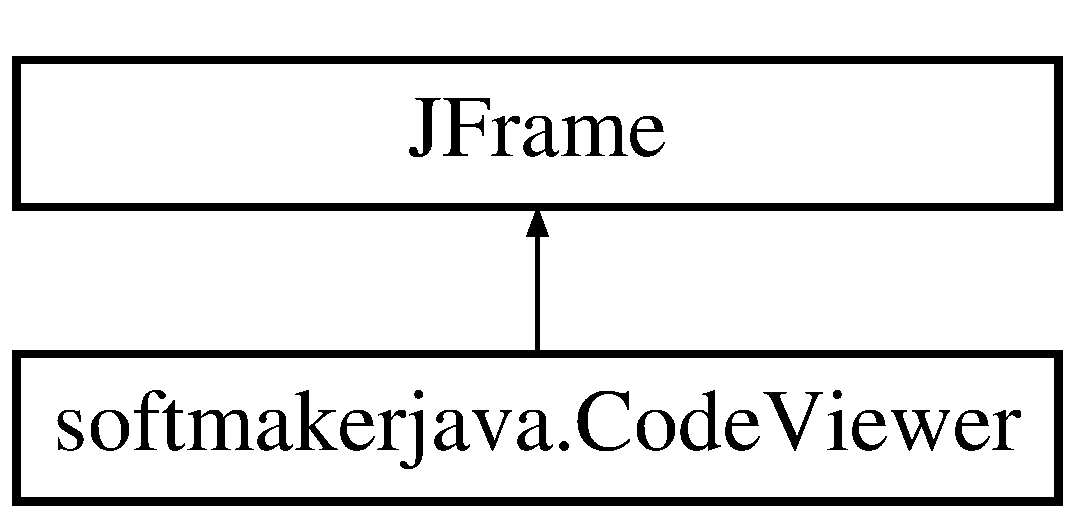
\includegraphics[height=2.000000cm]{classsoftmakerjava_1_1_code_viewer}
\end{center}
\end{figure}
\subsection*{Public Member Functions}
\begin{DoxyCompactItemize}
\item 
{\bfseries Code\+Viewer} (J\+Frame parent\+Frame)\hypertarget{classsoftmakerjava_1_1_code_viewer_a76900eb47a75cdba14fea5e5669dcb7d}{}\label{classsoftmakerjava_1_1_code_viewer_a76900eb47a75cdba14fea5e5669dcb7d}

\end{DoxyCompactItemize}
\subsection*{Private Member Functions}
\begin{DoxyCompactItemize}
\item 
void {\bfseries init\+Components} ()\hypertarget{classsoftmakerjava_1_1_code_viewer_a0c3534d1084e242bded8585487b32dbe}{}\label{classsoftmakerjava_1_1_code_viewer_a0c3534d1084e242bded8585487b32dbe}

\item 
void {\bfseries open\+But\+Action\+Performed} (java.\+awt.\+event.\+Action\+Event evt)\hypertarget{classsoftmakerjava_1_1_code_viewer_af1db1c71f1044d85109f1e4b512c360e}{}\label{classsoftmakerjava_1_1_code_viewer_af1db1c71f1044d85109f1e4b512c360e}

\item 
void {\bfseries form\+Window\+Closing} (java.\+awt.\+event.\+Window\+Event evt)\hypertarget{classsoftmakerjava_1_1_code_viewer_a8ea1263bbcd0338d23b29ae4dd8e13b8}{}\label{classsoftmakerjava_1_1_code_viewer_a8ea1263bbcd0338d23b29ae4dd8e13b8}

\item 
void {\bfseries save\+But\+Action\+Performed} (java.\+awt.\+event.\+Action\+Event evt)\hypertarget{classsoftmakerjava_1_1_code_viewer_a29588c8139784f46ac2acf13d8a154b6}{}\label{classsoftmakerjava_1_1_code_viewer_a29588c8139784f46ac2acf13d8a154b6}

\item 
void {\bfseries close\+But\+Action\+Performed} (java.\+awt.\+event.\+Action\+Event evt)\hypertarget{classsoftmakerjava_1_1_code_viewer_aeb4ee33f12dac276f4b70a42ff1bdbbb}{}\label{classsoftmakerjava_1_1_code_viewer_aeb4ee33f12dac276f4b70a42ff1bdbbb}

\item 
void {\bfseries new\+But\+Action\+Performed} (java.\+awt.\+event.\+Action\+Event evt)\hypertarget{classsoftmakerjava_1_1_code_viewer_a7bf4517277800150189170f601230d40}{}\label{classsoftmakerjava_1_1_code_viewer_a7bf4517277800150189170f601230d40}

\item 
void {\bfseries fill\+File\+List} ()\hypertarget{classsoftmakerjava_1_1_code_viewer_acaa7808ba411eef554e9c353e6cb4bd3}{}\label{classsoftmakerjava_1_1_code_viewer_acaa7808ba411eef554e9c353e6cb4bd3}

\end{DoxyCompactItemize}
\subsection*{Private Attributes}
\begin{DoxyCompactItemize}
\item 
final J\+Frame {\bfseries parent\+Frame}\hypertarget{classsoftmakerjava_1_1_code_viewer_a60a6852912ae36563ec8e0eed2676061}{}\label{classsoftmakerjava_1_1_code_viewer_a60a6852912ae36563ec8e0eed2676061}

\item 
\hyperlink{classsoftmakerjava_1_1_code_editor}{Code\+Editor} {\bfseries editor}\hypertarget{classsoftmakerjava_1_1_code_viewer_a6878b00fbd21f0823565fbf944213598}{}\label{classsoftmakerjava_1_1_code_viewer_a6878b00fbd21f0823565fbf944213598}

\item 
javax.\+swing.\+J\+Panel {\bfseries buttons1\+Panel}\hypertarget{classsoftmakerjava_1_1_code_viewer_a2441389ab6d45ab7b62b719a9d604c40}{}\label{classsoftmakerjava_1_1_code_viewer_a2441389ab6d45ab7b62b719a9d604c40}

\item 
javax.\+swing.\+J\+Panel {\bfseries buttons2\+Panel}\hypertarget{classsoftmakerjava_1_1_code_viewer_a7c1dc00a4c4ec7c448f6a5c9ee358d09}{}\label{classsoftmakerjava_1_1_code_viewer_a7c1dc00a4c4ec7c448f6a5c9ee358d09}

\item 
javax.\+swing.\+J\+Button {\bfseries close\+But}\hypertarget{classsoftmakerjava_1_1_code_viewer_a73730c28d3821a91a6bd410491bb23ce}{}\label{classsoftmakerjava_1_1_code_viewer_a73730c28d3821a91a6bd410491bb23ce}

\item 
javax.\+swing.\+J\+Text\+Area {\bfseries code\+Area}\hypertarget{classsoftmakerjava_1_1_code_viewer_a742d4d898a973ec856f5b8fa0c453669}{}\label{classsoftmakerjava_1_1_code_viewer_a742d4d898a973ec856f5b8fa0c453669}

\item 
javax.\+swing.\+J\+Combo\+Box {\bfseries files\+Combo}\hypertarget{classsoftmakerjava_1_1_code_viewer_aef6104a37c419a9fb6224628a2fa0bb6}{}\label{classsoftmakerjava_1_1_code_viewer_aef6104a37c419a9fb6224628a2fa0bb6}

\item 
javax.\+swing.\+J\+Scroll\+Pane {\bfseries j\+Scroll\+Pane1}\hypertarget{classsoftmakerjava_1_1_code_viewer_aa37978c1591b5972ec611584ef132e9f}{}\label{classsoftmakerjava_1_1_code_viewer_aa37978c1591b5972ec611584ef132e9f}

\item 
javax.\+swing.\+J\+Button {\bfseries new\+But}\hypertarget{classsoftmakerjava_1_1_code_viewer_ae3c60ae3cb920aecedb229604ac24ddd}{}\label{classsoftmakerjava_1_1_code_viewer_ae3c60ae3cb920aecedb229604ac24ddd}

\item 
javax.\+swing.\+J\+Button {\bfseries open\+But}\hypertarget{classsoftmakerjava_1_1_code_viewer_a3a473b4efc1d636a7a87869898f3549f}{}\label{classsoftmakerjava_1_1_code_viewer_a3a473b4efc1d636a7a87869898f3549f}

\item 
javax.\+swing.\+J\+Button {\bfseries save\+But}\hypertarget{classsoftmakerjava_1_1_code_viewer_a8943cf8b2795897c465ee07f473e92e2}{}\label{classsoftmakerjava_1_1_code_viewer_a8943cf8b2795897c465ee07f473e92e2}

\end{DoxyCompactItemize}


\subsection{Detailed Description}
\begin{DoxyAuthor}{Author}
Baka 
\end{DoxyAuthor}


The documentation for this class was generated from the following file\+:\begin{DoxyCompactItemize}
\item 
C\+:/\+Users/\+Wojtek\+K/\+Desktop/\+Soft\+Maker\+Java1/src/softmakerjava/Code\+Viewer.\+java\end{DoxyCompactItemize}

\hypertarget{classsoftmakerjava_1_1_employee_panel}{}\section{softmakerjava.\+Employee\+Panel Class Reference}
\label{classsoftmakerjava_1_1_employee_panel}\index{softmakerjava.\+Employee\+Panel@{softmakerjava.\+Employee\+Panel}}
\subsection*{Private Member Functions}
\begin{DoxyCompactItemize}
\item 
void {\bfseries generate\+G\+UI} ()\hypertarget{classsoftmakerjava_1_1_employee_panel_a65a82e401bef7e5fefbe1e3d514583f9}{}\label{classsoftmakerjava_1_1_employee_panel_a65a82e401bef7e5fefbe1e3d514583f9}

\end{DoxyCompactItemize}
\subsection*{Private Attributes}
\begin{DoxyCompactItemize}
\item 
J\+Frame {\bfseries main\+Frame}\hypertarget{classsoftmakerjava_1_1_employee_panel_a2485a0dd32b74a75903f3abb4d6b2947}{}\label{classsoftmakerjava_1_1_employee_panel_a2485a0dd32b74a75903f3abb4d6b2947}

\item 
J\+Label {\bfseries TaskL}\hypertarget{classsoftmakerjava_1_1_employee_panel_a2c0695a415bb394696e30f8845e0560e}{}\label{classsoftmakerjava_1_1_employee_panel_a2c0695a415bb394696e30f8845e0560e}

\item 
J\+Combo\+Box {\bfseries Tasks}\hypertarget{classsoftmakerjava_1_1_employee_panel_a3439b96e80f6d72bc6df0df0da25dece}{}\label{classsoftmakerjava_1_1_employee_panel_a3439b96e80f6d72bc6df0df0da25dece}

\item 
J\+Button {\bfseries Deploy\+Task}\hypertarget{classsoftmakerjava_1_1_employee_panel_ac56fb2347a9d62e8a3c6b90cdf648ad5}{}\label{classsoftmakerjava_1_1_employee_panel_ac56fb2347a9d62e8a3c6b90cdf648ad5}

\item 
J\+Button {\bfseries User\+Tasks}\hypertarget{classsoftmakerjava_1_1_employee_panel_a6a84141fc2fc2c3806d180394c9d95ed}{}\label{classsoftmakerjava_1_1_employee_panel_a6a84141fc2fc2c3806d180394c9d95ed}

\end{DoxyCompactItemize}


The documentation for this class was generated from the following file\+:\begin{DoxyCompactItemize}
\item 
C\+:/\+Users/\+Wojtek\+K/\+Desktop/\+Soft\+Maker\+Java1/src/softmakerjava/Employee\+Panel.\+java\end{DoxyCompactItemize}

\hypertarget{classsoftmakerjava_1_1_general_settings_editor}{}\section{softmakerjava.\+General\+Settings\+Editor Class Reference}
\label{classsoftmakerjava_1_1_general_settings_editor}\index{softmakerjava.\+General\+Settings\+Editor@{softmakerjava.\+General\+Settings\+Editor}}
\subsection*{Static Public Attributes}
\begin{DoxyCompactItemize}
\item 
static \hyperlink{classsoftmakerjava_1_1_settings}{Settings} {\bfseries settings}\hypertarget{classsoftmakerjava_1_1_general_settings_editor_adb0741d1b90e277f06ae10823264973c}{}\label{classsoftmakerjava_1_1_general_settings_editor_adb0741d1b90e277f06ae10823264973c}

\item 
static \hyperlink{classsoftmakerjava_1_1_user}{User} {\bfseries current\+User}\hypertarget{classsoftmakerjava_1_1_general_settings_editor_a62291204138033e59c2f87e317e59a90}{}\label{classsoftmakerjava_1_1_general_settings_editor_a62291204138033e59c2f87e317e59a90}

\end{DoxyCompactItemize}
\subsection*{Static Protected Member Functions}
\begin{DoxyCompactItemize}
\item 
static void {\bfseries change\+Language} (String lang)\hypertarget{classsoftmakerjava_1_1_general_settings_editor_a26f9dd0c0342e02e5a5731832e967ffa}{}\label{classsoftmakerjava_1_1_general_settings_editor_a26f9dd0c0342e02e5a5731832e967ffa}

\item 
static boolean {\bfseries save\+Settings} (String code\+Language, String language, String server\+IP, Integer server\+Port)\hypertarget{classsoftmakerjava_1_1_general_settings_editor_ae16606b6644d56e68e1cf909576d22f5}{}\label{classsoftmakerjava_1_1_general_settings_editor_ae16606b6644d56e68e1cf909576d22f5}

\item 
static void {\bfseries load\+Settings} ()\hypertarget{classsoftmakerjava_1_1_general_settings_editor_ae12dad63b8bc506d97dfdae617f89672}{}\label{classsoftmakerjava_1_1_general_settings_editor_ae12dad63b8bc506d97dfdae617f89672}

\item 
static void {\bfseries reset\+To\+Default} ()\hypertarget{classsoftmakerjava_1_1_general_settings_editor_ab68ece24d8b52b3461b5d994e605ddce}{}\label{classsoftmakerjava_1_1_general_settings_editor_ab68ece24d8b52b3461b5d994e605ddce}

\end{DoxyCompactItemize}
\subsection*{Static Private Member Functions}
\begin{DoxyCompactItemize}
\item 
static void {\bfseries set\+Up\+Connection} ()\hypertarget{classsoftmakerjava_1_1_general_settings_editor_a584645fd6b751e05b44280b2f16bc5c6}{}\label{classsoftmakerjava_1_1_general_settings_editor_a584645fd6b751e05b44280b2f16bc5c6}

\item 
static void {\bfseries close\+Connection} ()\hypertarget{classsoftmakerjava_1_1_general_settings_editor_a29fed609b53c82a4255ada48c13f6d75}{}\label{classsoftmakerjava_1_1_general_settings_editor_a29fed609b53c82a4255ada48c13f6d75}

\end{DoxyCompactItemize}
\subsection*{Static Private Attributes}
\begin{DoxyCompactItemize}
\item 
static Connection {\bfseries server\+Connection}\hypertarget{classsoftmakerjava_1_1_general_settings_editor_ab4268229813c48546dd946cc9cd5b9cc}{}\label{classsoftmakerjava_1_1_general_settings_editor_ab4268229813c48546dd946cc9cd5b9cc}

\end{DoxyCompactItemize}


\subsection{Detailed Description}
\begin{DoxyAuthor}{Author}
Baka 
\end{DoxyAuthor}


The documentation for this class was generated from the following file\+:\begin{DoxyCompactItemize}
\item 
C\+:/\+Users/\+Wojtek\+K/\+Desktop/\+Soft\+Maker\+Java1/src/softmakerjava/General\+Settings\+Editor.\+java\end{DoxyCompactItemize}

\hypertarget{classsoftmakerjava_1_1_info_center}{}\section{softmakerjava.\+Info\+Center Class Reference}
\label{classsoftmakerjava_1_1_info_center}\index{softmakerjava.\+Info\+Center@{softmakerjava.\+Info\+Center}}
\subsection*{Public Member Functions}
\begin{DoxyCompactItemize}
\item 
\hyperlink{classsoftmakerjava_1_1_user}{User} {\bfseries get\+Current\+User} ()\hypertarget{classsoftmakerjava_1_1_info_center_a6350ea9cb7a0fea7ba40ac4d8221043c}{}\label{classsoftmakerjava_1_1_info_center_a6350ea9cb7a0fea7ba40ac4d8221043c}

\item 
void {\bfseries set\+Current\+User} (\hyperlink{classsoftmakerjava_1_1_user}{User} current\+User)\hypertarget{classsoftmakerjava_1_1_info_center_acab3307193c7761a3a25466c0e439b1f}{}\label{classsoftmakerjava_1_1_info_center_acab3307193c7761a3a25466c0e439b1f}

\end{DoxyCompactItemize}


The documentation for this class was generated from the following file\+:\begin{DoxyCompactItemize}
\item 
C\+:/\+Users/\+Wojtek\+K/\+Desktop/\+Soft\+Maker\+Java1/src/softmakerjava/Info\+Center.\+java\end{DoxyCompactItemize}

\hypertarget{classsoftmakerjava_1_1_login_form}{}\section{softmakerjava.\+Login\+Form Class Reference}
\label{classsoftmakerjava_1_1_login_form}\index{softmakerjava.\+Login\+Form@{softmakerjava.\+Login\+Form}}
Inheritance diagram for softmakerjava.\+Login\+Form\+:\begin{figure}[H]
\begin{center}
\leavevmode
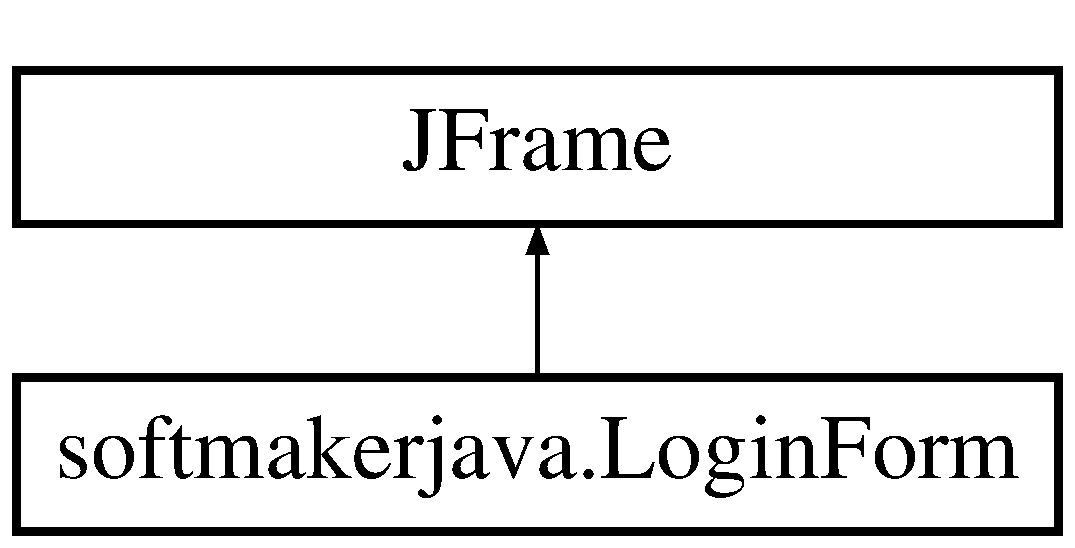
\includegraphics[height=2.000000cm]{classsoftmakerjava_1_1_login_form}
\end{center}
\end{figure}
\subsection*{Private Member Functions}
\begin{DoxyCompactItemize}
\item 
void {\bfseries init\+Components} ()\hypertarget{classsoftmakerjava_1_1_login_form_aa525caaa4005a23182f277fa7969968d}{}\label{classsoftmakerjava_1_1_login_form_aa525caaa4005a23182f277fa7969968d}

\item 
void {\bfseries username\+Field\+Action\+Performed} (java.\+awt.\+event.\+Action\+Event evt)\hypertarget{classsoftmakerjava_1_1_login_form_a4c5c894c2161d64ba97f7294ad16b4ea}{}\label{classsoftmakerjava_1_1_login_form_a4c5c894c2161d64ba97f7294ad16b4ea}

\item 
void {\bfseries login\+Button\+Mouse\+Clicked} (java.\+awt.\+event.\+Mouse\+Event evt)\hypertarget{classsoftmakerjava_1_1_login_form_a3ca2528a35be8b1e4f665481da171fe8}{}\label{classsoftmakerjava_1_1_login_form_a3ca2528a35be8b1e4f665481da171fe8}

\item 
void {\bfseries login\+Action} (\hyperlink{classsoftmakerjava_1_1_user}{User} user\+Obj)\hypertarget{classsoftmakerjava_1_1_login_form_ac469ebbf9a6341fc4bb7825c6b1b51a1}{}\label{classsoftmakerjava_1_1_login_form_ac469ebbf9a6341fc4bb7825c6b1b51a1}

\end{DoxyCompactItemize}
\subsection*{Private Attributes}
\begin{DoxyCompactItemize}
\item 
Array\+List$<$ \hyperlink{classsoftmakerjava_1_1_user}{User} $>$ {\bfseries user\+List}\hypertarget{classsoftmakerjava_1_1_login_form_ae174d7c341fc040d7ada34a7fd529d63}{}\label{classsoftmakerjava_1_1_login_form_ae174d7c341fc040d7ada34a7fd529d63}

\item 
javax.\+swing.\+J\+Label {\bfseries info\+Label}\hypertarget{classsoftmakerjava_1_1_login_form_a3ffd9fed6d9a3ab5cc7dcc5515e17417}{}\label{classsoftmakerjava_1_1_login_form_a3ffd9fed6d9a3ab5cc7dcc5515e17417}

\item 
javax.\+swing.\+J\+Button {\bfseries login\+Button}\hypertarget{classsoftmakerjava_1_1_login_form_a7fa501ae873a8a60b2cc7c04462d7893}{}\label{classsoftmakerjava_1_1_login_form_a7fa501ae873a8a60b2cc7c04462d7893}

\item 
javax.\+swing.\+J\+Panel {\bfseries login\+Componenets\+Panel}\hypertarget{classsoftmakerjava_1_1_login_form_a3c99b03811013db337563a9ee035263f}{}\label{classsoftmakerjava_1_1_login_form_a3c99b03811013db337563a9ee035263f}

\item 
javax.\+swing.\+J\+Text\+Field {\bfseries username\+Field}\hypertarget{classsoftmakerjava_1_1_login_form_a7abc2803be9aba93267fb2b3bbe3835f}{}\label{classsoftmakerjava_1_1_login_form_a7abc2803be9aba93267fb2b3bbe3835f}

\end{DoxyCompactItemize}


\subsection{Detailed Description}
\begin{DoxyAuthor}{Author}
Baka 
\end{DoxyAuthor}


The documentation for this class was generated from the following file\+:\begin{DoxyCompactItemize}
\item 
C\+:/\+Users/\+Wojtek\+K/\+Desktop/\+Soft\+Maker\+Java1/src/softmakerjava/Login\+Form.\+java\end{DoxyCompactItemize}

\hypertarget{classsoftmakerjava_1_1_main_frame}{}\section{softmakerjava.\+Main\+Frame Class Reference}
\label{classsoftmakerjava_1_1_main_frame}\index{softmakerjava.\+Main\+Frame@{softmakerjava.\+Main\+Frame}}
Inheritance diagram for softmakerjava.\+Main\+Frame\+:\begin{figure}[H]
\begin{center}
\leavevmode
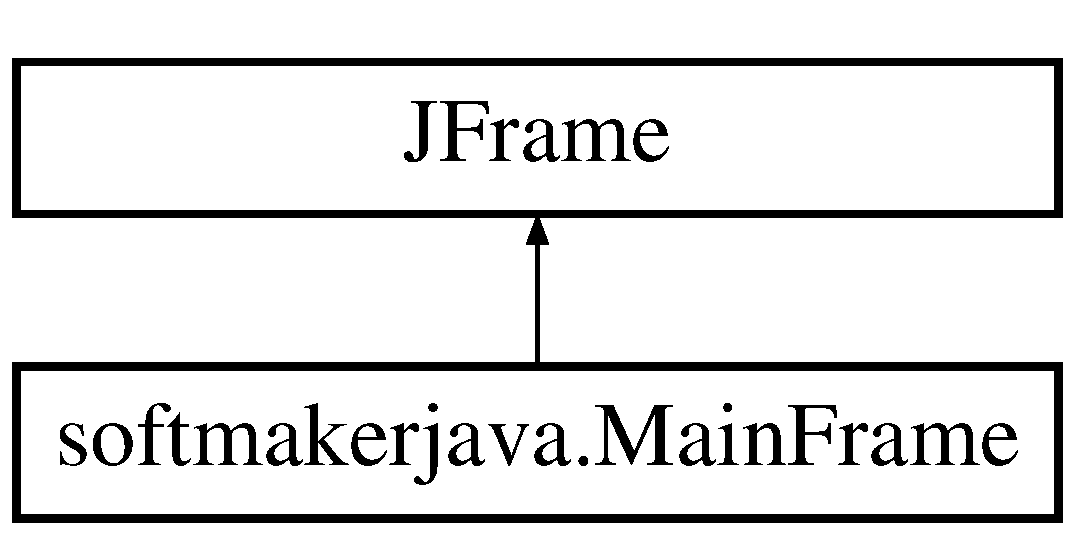
\includegraphics[height=2.000000cm]{classsoftmakerjava_1_1_main_frame}
\end{center}
\end{figure}
\subsection*{Public Member Functions}
\begin{DoxyCompactItemize}
\item 
{\bfseries Main\+Frame} (\hyperlink{classsoftmakerjava_1_1_user}{User} user)\hypertarget{classsoftmakerjava_1_1_main_frame_a10aa668ac3039183b2a1865374aa0fcf}{}\label{classsoftmakerjava_1_1_main_frame_a10aa668ac3039183b2a1865374aa0fcf}

\end{DoxyCompactItemize}
\subsection*{Private Member Functions}
\begin{DoxyCompactItemize}
\item 
void \hyperlink{classsoftmakerjava_1_1_main_frame_a527cea1a1e0cc8bd5497aaf4ada1c50e}{init\+Components} ()
\item 
void {\bfseries own\+Init} ()\hypertarget{classsoftmakerjava_1_1_main_frame_aa62d2fe0f6ccdb8066c6b085eedcd52d}{}\label{classsoftmakerjava_1_1_main_frame_aa62d2fe0f6ccdb8066c6b085eedcd52d}

\end{DoxyCompactItemize}
\subsection*{Private Attributes}
\begin{DoxyCompactItemize}
\item 
javax.\+swing.\+J\+Panel {\bfseries Header\+Panel}\hypertarget{classsoftmakerjava_1_1_main_frame_aa343c9ded9d888efa9865938cfff4302}{}\label{classsoftmakerjava_1_1_main_frame_aa343c9ded9d888efa9865938cfff4302}

\item 
javax.\+swing.\+J\+Panel {\bfseries Menu\+Panel}\hypertarget{classsoftmakerjava_1_1_main_frame_a1d556bb82806724cf06f2f75ce1bdaa3}{}\label{classsoftmakerjava_1_1_main_frame_a1d556bb82806724cf06f2f75ce1bdaa3}

\item 
javax.\+swing.\+J\+Label {\bfseries code\+Editor\+Label}\hypertarget{classsoftmakerjava_1_1_main_frame_a3958ea946601a4a142db60cc0503e0b7}{}\label{classsoftmakerjava_1_1_main_frame_a3958ea946601a4a142db60cc0503e0b7}

\item 
javax.\+swing.\+J\+Label {\bfseries employe\+Panel}\hypertarget{classsoftmakerjava_1_1_main_frame_a793b3402a0fce11e49ac9043c04c75a8}{}\label{classsoftmakerjava_1_1_main_frame_a793b3402a0fce11e49ac9043c04c75a8}

\item 
javax.\+swing.\+J\+Panel {\bfseries j\+Panel1}\hypertarget{classsoftmakerjava_1_1_main_frame_a33cb8ae9084ddc738dba3ea355c3d586}{}\label{classsoftmakerjava_1_1_main_frame_a33cb8ae9084ddc738dba3ea355c3d586}

\item 
javax.\+swing.\+J\+Label {\bfseries server\+Acess\+Panel}\hypertarget{classsoftmakerjava_1_1_main_frame_a90facb5fe865ed4d8bfa652492a9e728}{}\label{classsoftmakerjava_1_1_main_frame_a90facb5fe865ed4d8bfa652492a9e728}

\item 
javax.\+swing.\+J\+Label {\bfseries settings\+Panel\+Label}\hypertarget{classsoftmakerjava_1_1_main_frame_ab6f360e499fce226b430d833a3b83641}{}\label{classsoftmakerjava_1_1_main_frame_ab6f360e499fce226b430d833a3b83641}

\item 
javax.\+swing.\+J\+Label {\bfseries task\+Panel}\hypertarget{classsoftmakerjava_1_1_main_frame_a56e27e0ecf317544df1c2a3f27e0e503}{}\label{classsoftmakerjava_1_1_main_frame_a56e27e0ecf317544df1c2a3f27e0e503}

\item 
javax.\+swing.\+J\+Label {\bfseries username\+Label}\hypertarget{classsoftmakerjava_1_1_main_frame_a571fdaab46094e8a5adec43dc8ac5505}{}\label{classsoftmakerjava_1_1_main_frame_a571fdaab46094e8a5adec43dc8ac5505}

\end{DoxyCompactItemize}


\subsection{Detailed Description}
\begin{DoxyAuthor}{Author}
Baka 
\end{DoxyAuthor}


\subsection{Member Function Documentation}
\index{softmakerjava\+::\+Main\+Frame@{softmakerjava\+::\+Main\+Frame}!init\+Components@{init\+Components}}
\index{init\+Components@{init\+Components}!softmakerjava\+::\+Main\+Frame@{softmakerjava\+::\+Main\+Frame}}
\subsubsection[{\texorpdfstring{init\+Components()}{initComponents()}}]{\setlength{\rightskip}{0pt plus 5cm}void softmakerjava.\+Main\+Frame.\+init\+Components (
\begin{DoxyParamCaption}
{}
\end{DoxyParamCaption}
)\hspace{0.3cm}{\ttfamily [private]}}\hypertarget{classsoftmakerjava_1_1_main_frame_a527cea1a1e0cc8bd5497aaf4ada1c50e}{}\label{classsoftmakerjava_1_1_main_frame_a527cea1a1e0cc8bd5497aaf4ada1c50e}
This method is called from within the constructor to initialize the form. W\+A\+R\+N\+I\+NG\+: Do N\+OT modify this code. The content of this method is always regenerated by the Form Editor. 

The documentation for this class was generated from the following file\+:\begin{DoxyCompactItemize}
\item 
C\+:/\+Users/\+Wojtek\+K/\+Desktop/\+Soft\+Maker\+Java1/src/softmakerjava/Main\+Frame.\+java\end{DoxyCompactItemize}

\hypertarget{classsoftmakerjava_1_1_manager_center}{}\section{softmakerjava.\+Manager\+Center Class Reference}
\label{classsoftmakerjava_1_1_manager_center}\index{softmakerjava.\+Manager\+Center@{softmakerjava.\+Manager\+Center}}
\subsection*{Public Member Functions}
\begin{DoxyCompactItemize}
\item 
Vector {\bfseries Get\+User\+List} ()\hypertarget{classsoftmakerjava_1_1_manager_center_a24a47d603a8c18d90d12e22e699c34f7}{}\label{classsoftmakerjava_1_1_manager_center_a24a47d603a8c18d90d12e22e699c34f7}

\end{DoxyCompactItemize}


The documentation for this class was generated from the following file\+:\begin{DoxyCompactItemize}
\item 
C\+:/\+Users/\+Wojtek\+K/\+Desktop/\+Soft\+Maker\+Java1/src/softmakerjava/Manager\+Center.\+java\end{DoxyCompactItemize}

\hypertarget{classsoftmakerjava_1_1_server_acess_window}{}\section{softmakerjava.\+Server\+Acess\+Window Class Reference}
\label{classsoftmakerjava_1_1_server_acess_window}\index{softmakerjava.\+Server\+Acess\+Window@{softmakerjava.\+Server\+Acess\+Window}}
Inheritance diagram for softmakerjava.\+Server\+Acess\+Window\+:\begin{figure}[H]
\begin{center}
\leavevmode
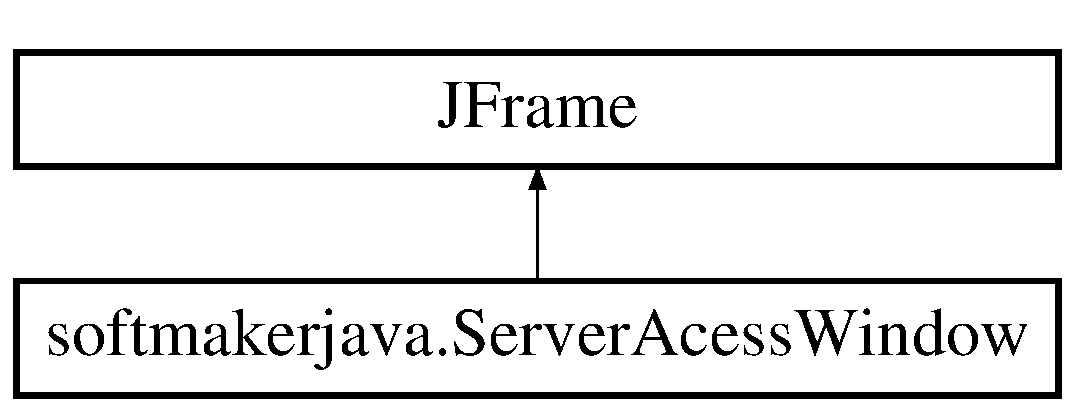
\includegraphics[height=2.000000cm]{classsoftmakerjava_1_1_server_acess_window}
\end{center}
\end{figure}
\subsection*{Public Member Functions}
\begin{DoxyCompactItemize}
\item 
{\bfseries Server\+Acess\+Window} (J\+Frame parent\+Frame)\hypertarget{classsoftmakerjava_1_1_server_acess_window_ad5cb90a42f6cf9dcc29f0e9e7d341d15}{}\label{classsoftmakerjava_1_1_server_acess_window_ad5cb90a42f6cf9dcc29f0e9e7d341d15}

\end{DoxyCompactItemize}
\subsection*{Private Member Functions}
\begin{DoxyCompactItemize}
\item 
void {\bfseries init\+Components} ()\hypertarget{classsoftmakerjava_1_1_server_acess_window_a17c487bed9b33025000e008bc090b210}{}\label{classsoftmakerjava_1_1_server_acess_window_a17c487bed9b33025000e008bc090b210}

\item 
void {\bfseries form\+Window\+Closing} (java.\+awt.\+event.\+Window\+Event evt)\hypertarget{classsoftmakerjava_1_1_server_acess_window_a2778345682cad85f7dd163498a58d748}{}\label{classsoftmakerjava_1_1_server_acess_window_a2778345682cad85f7dd163498a58d748}

\item 
void {\bfseries reload\+But\+Action\+Performed} (java.\+awt.\+event.\+Action\+Event evt)\hypertarget{classsoftmakerjava_1_1_server_acess_window_a431199141b312e6f39d96225c645fc31}{}\label{classsoftmakerjava_1_1_server_acess_window_a431199141b312e6f39d96225c645fc31}

\item 
void {\bfseries del\+File\+But\+Action\+Performed} (java.\+awt.\+event.\+Action\+Event evt)\hypertarget{classsoftmakerjava_1_1_server_acess_window_a8993db864d7bf095f70127ba4c22eda5}{}\label{classsoftmakerjava_1_1_server_acess_window_a8993db864d7bf095f70127ba4c22eda5}

\item 
void {\bfseries new\+File\+But\+Action\+Performed} (java.\+awt.\+event.\+Action\+Event evt)\hypertarget{classsoftmakerjava_1_1_server_acess_window_a67b8d1cc83b791ee20cf43654fdb1e7e}{}\label{classsoftmakerjava_1_1_server_acess_window_a67b8d1cc83b791ee20cf43654fdb1e7e}

\item 
void {\bfseries fill\+File\+List} ()\hypertarget{classsoftmakerjava_1_1_server_acess_window_a7cadc87f7de1f1c1c7095c59310a1f0f}{}\label{classsoftmakerjava_1_1_server_acess_window_a7cadc87f7de1f1c1c7095c59310a1f0f}

\end{DoxyCompactItemize}
\subsection*{Private Attributes}
\begin{DoxyCompactItemize}
\item 
final J\+Frame {\bfseries parent\+Frame}\hypertarget{classsoftmakerjava_1_1_server_acess_window_a07c4ae5c4390b19edfc27aa9f23910cf}{}\label{classsoftmakerjava_1_1_server_acess_window_a07c4ae5c4390b19edfc27aa9f23910cf}

\item 
javax.\+swing.\+J\+Button {\bfseries del\+File\+But}\hypertarget{classsoftmakerjava_1_1_server_acess_window_ab167c871b1f3d16f6eca0240cdb83763}{}\label{classsoftmakerjava_1_1_server_acess_window_ab167c871b1f3d16f6eca0240cdb83763}

\item 
javax.\+swing.\+J\+Text\+Field {\bfseries filename\+Field}\hypertarget{classsoftmakerjava_1_1_server_acess_window_a6cf031efd4e4f73e50086a05a0871ede}{}\label{classsoftmakerjava_1_1_server_acess_window_a6cf031efd4e4f73e50086a05a0871ede}

\item 
javax.\+swing.\+J\+List {\bfseries files\+List}\hypertarget{classsoftmakerjava_1_1_server_acess_window_a2901a45288def92016e3a9beec51497e}{}\label{classsoftmakerjava_1_1_server_acess_window_a2901a45288def92016e3a9beec51497e}

\item 
javax.\+swing.\+J\+Label {\bfseries files\+List\+Label}\hypertarget{classsoftmakerjava_1_1_server_acess_window_a6545d3f8c2e9f4bd5a05880f387375bf}{}\label{classsoftmakerjava_1_1_server_acess_window_a6545d3f8c2e9f4bd5a05880f387375bf}

\item 
javax.\+swing.\+J\+Scroll\+Pane {\bfseries files\+Scroll\+Panel}\hypertarget{classsoftmakerjava_1_1_server_acess_window_a24db52aba1236e32cc2972777d842e73}{}\label{classsoftmakerjava_1_1_server_acess_window_a24db52aba1236e32cc2972777d842e73}

\item 
javax.\+swing.\+J\+Panel {\bfseries j\+Panel1}\hypertarget{classsoftmakerjava_1_1_server_acess_window_a5aea81daf6bf685a9252486afab92705}{}\label{classsoftmakerjava_1_1_server_acess_window_a5aea81daf6bf685a9252486afab92705}

\item 
javax.\+swing.\+J\+Button {\bfseries new\+File\+But}\hypertarget{classsoftmakerjava_1_1_server_acess_window_a878d8d9498b15422052f5bf9211e82e7}{}\label{classsoftmakerjava_1_1_server_acess_window_a878d8d9498b15422052f5bf9211e82e7}

\item 
javax.\+swing.\+J\+Button {\bfseries reload\+But}\hypertarget{classsoftmakerjava_1_1_server_acess_window_ab8cc71a6c57b732eed65c1f21cb264a0}{}\label{classsoftmakerjava_1_1_server_acess_window_ab8cc71a6c57b732eed65c1f21cb264a0}

\end{DoxyCompactItemize}


\subsection{Detailed Description}
\begin{DoxyAuthor}{Author}
Baka 
\end{DoxyAuthor}


The documentation for this class was generated from the following file\+:\begin{DoxyCompactItemize}
\item 
C\+:/\+Users/\+Wojtek\+K/\+Desktop/\+Soft\+Maker\+Java1/src/softmakerjava/Server\+Acess\+Window.\+java\end{DoxyCompactItemize}

\hypertarget{classsoftmakerjava_1_1_server_handler}{}\section{softmakerjava.\+Server\+Handler Class Reference}
\label{classsoftmakerjava_1_1_server_handler}\index{softmakerjava.\+Server\+Handler@{softmakerjava.\+Server\+Handler}}
\subsection*{Static Protected Member Functions}
\begin{DoxyCompactItemize}
\item 
static Boolean {\bfseries save\+On\+Server} (File file, String file\+Name)\hypertarget{classsoftmakerjava_1_1_server_handler_a189f9439b9c3757851f903d68e38f9f8}{}\label{classsoftmakerjava_1_1_server_handler_a189f9439b9c3757851f903d68e38f9f8}

\item 
static File {\bfseries load\+From\+Server} (String file\+Name)\hypertarget{classsoftmakerjava_1_1_server_handler_ad4b1765682cc3f98aadd549892bd80df}{}\label{classsoftmakerjava_1_1_server_handler_ad4b1765682cc3f98aadd549892bd80df}

\item 
static Boolean {\bfseries delete\+From\+Server} (String file\+Name)\hypertarget{classsoftmakerjava_1_1_server_handler_a9e9a3bdc1b864c2cd596850531fa1c2e}{}\label{classsoftmakerjava_1_1_server_handler_a9e9a3bdc1b864c2cd596850531fa1c2e}

\item 
static Array\+List$<$ String $>$ {\bfseries get\+File\+Titles} ()\hypertarget{classsoftmakerjava_1_1_server_handler_a74c93c88f6cc0eb8b49c5423e864c874}{}\label{classsoftmakerjava_1_1_server_handler_a74c93c88f6cc0eb8b49c5423e864c874}

\end{DoxyCompactItemize}
\subsection*{Static Private Member Functions}
\begin{DoxyCompactItemize}
\item 
static void {\bfseries set\+Up\+Connection} ()\hypertarget{classsoftmakerjava_1_1_server_handler_a76dc38beb484cbe4bb361789e627e3fe}{}\label{classsoftmakerjava_1_1_server_handler_a76dc38beb484cbe4bb361789e627e3fe}

\item 
static void {\bfseries close\+Connection} ()\hypertarget{classsoftmakerjava_1_1_server_handler_a510669855864af0d1d6a564bc070343c}{}\label{classsoftmakerjava_1_1_server_handler_a510669855864af0d1d6a564bc070343c}

\end{DoxyCompactItemize}
\subsection*{Static Private Attributes}
\begin{DoxyCompactItemize}
\item 
static Connection {\bfseries server\+Connection}\hypertarget{classsoftmakerjava_1_1_server_handler_aac99fbd5c63a9d9a9225c9f356e55830}{}\label{classsoftmakerjava_1_1_server_handler_aac99fbd5c63a9d9a9225c9f356e55830}

\end{DoxyCompactItemize}


\subsection{Detailed Description}
\begin{DoxyAuthor}{Author}
Baka 
\end{DoxyAuthor}


The documentation for this class was generated from the following file\+:\begin{DoxyCompactItemize}
\item 
C\+:/\+Users/\+Wojtek\+K/\+Desktop/\+Soft\+Maker\+Java1/src/softmakerjava/Server\+Handler.\+java\end{DoxyCompactItemize}

\hypertarget{classsoftmakerjava_1_1_settings}{}\section{softmakerjava.\+Settings Class Reference}
\label{classsoftmakerjava_1_1_settings}\index{softmakerjava.\+Settings@{softmakerjava.\+Settings}}
\subsection*{Public Member Functions}
\begin{DoxyCompactItemize}
\item 
String {\bfseries get\+Language} ()\hypertarget{classsoftmakerjava_1_1_settings_a058521f262df4c1399d496da81ab89a5}{}\label{classsoftmakerjava_1_1_settings_a058521f262df4c1399d496da81ab89a5}

\item 
void {\bfseries set\+Language} (String Language)\hypertarget{classsoftmakerjava_1_1_settings_ad48a2cf35ccfa7f69682c581683800ac}{}\label{classsoftmakerjava_1_1_settings_ad48a2cf35ccfa7f69682c581683800ac}

\item 
String {\bfseries get\+Code\+Language} ()\hypertarget{classsoftmakerjava_1_1_settings_a887aad4d91579cd1ab6f831bbaa43be8}{}\label{classsoftmakerjava_1_1_settings_a887aad4d91579cd1ab6f831bbaa43be8}

\item 
void {\bfseries set\+Code\+Language} (String Code\+Language)\hypertarget{classsoftmakerjava_1_1_settings_a4b47b47adbc0b4df7270190eba9a9b34}{}\label{classsoftmakerjava_1_1_settings_a4b47b47adbc0b4df7270190eba9a9b34}

\item 
String {\bfseries get\+Server\+IP} ()\hypertarget{classsoftmakerjava_1_1_settings_abfe64adb52fd010b00c708a8604406b8}{}\label{classsoftmakerjava_1_1_settings_abfe64adb52fd010b00c708a8604406b8}

\item 
void {\bfseries set\+Server\+IP} (String Server\+IP)\hypertarget{classsoftmakerjava_1_1_settings_a6ad428542d1ecda64f41eef635a93b0c}{}\label{classsoftmakerjava_1_1_settings_a6ad428542d1ecda64f41eef635a93b0c}

\item 
int {\bfseries get\+Server\+Port} ()\hypertarget{classsoftmakerjava_1_1_settings_aa4c941689fa177441994a59118782729}{}\label{classsoftmakerjava_1_1_settings_aa4c941689fa177441994a59118782729}

\item 
void {\bfseries set\+Server\+Port} (int Server\+Port)\hypertarget{classsoftmakerjava_1_1_settings_a33c87cc25d677e70a9be56ee43c2e88a}{}\label{classsoftmakerjava_1_1_settings_a33c87cc25d677e70a9be56ee43c2e88a}

\end{DoxyCompactItemize}
\subsection*{Private Attributes}
\begin{DoxyCompactItemize}
\item 
String {\bfseries Language}\hypertarget{classsoftmakerjava_1_1_settings_a1d426ec86b5b7c0ef4dffdb4f2a5583d}{}\label{classsoftmakerjava_1_1_settings_a1d426ec86b5b7c0ef4dffdb4f2a5583d}

\item 
String {\bfseries Code\+Language}\hypertarget{classsoftmakerjava_1_1_settings_a2f84d3c56224d3e38da239a2461ee6da}{}\label{classsoftmakerjava_1_1_settings_a2f84d3c56224d3e38da239a2461ee6da}

\item 
String {\bfseries Server\+IP}\hypertarget{classsoftmakerjava_1_1_settings_a4ae12ca7cfc3eaccec1fe0b005de71a2}{}\label{classsoftmakerjava_1_1_settings_a4ae12ca7cfc3eaccec1fe0b005de71a2}

\item 
int {\bfseries Server\+Port}\hypertarget{classsoftmakerjava_1_1_settings_a4730f3da93d2d4f792fff7bac3f2a6fc}{}\label{classsoftmakerjava_1_1_settings_a4730f3da93d2d4f792fff7bac3f2a6fc}

\end{DoxyCompactItemize}


\subsection{Detailed Description}
\begin{DoxyAuthor}{Author}
Baka 
\end{DoxyAuthor}


The documentation for this class was generated from the following file\+:\begin{DoxyCompactItemize}
\item 
C\+:/\+Users/\+Wojtek\+K/\+Desktop/\+Soft\+Maker\+Java1/src/softmakerjava/Settings.\+java\end{DoxyCompactItemize}

\hypertarget{classsoftmakerjava_1_1_settings_panel}{}\section{softmakerjava.\+Settings\+Panel Class Reference}
\label{classsoftmakerjava_1_1_settings_panel}\index{softmakerjava.\+Settings\+Panel@{softmakerjava.\+Settings\+Panel}}
Inheritance diagram for softmakerjava.\+Settings\+Panel\+:\begin{figure}[H]
\begin{center}
\leavevmode
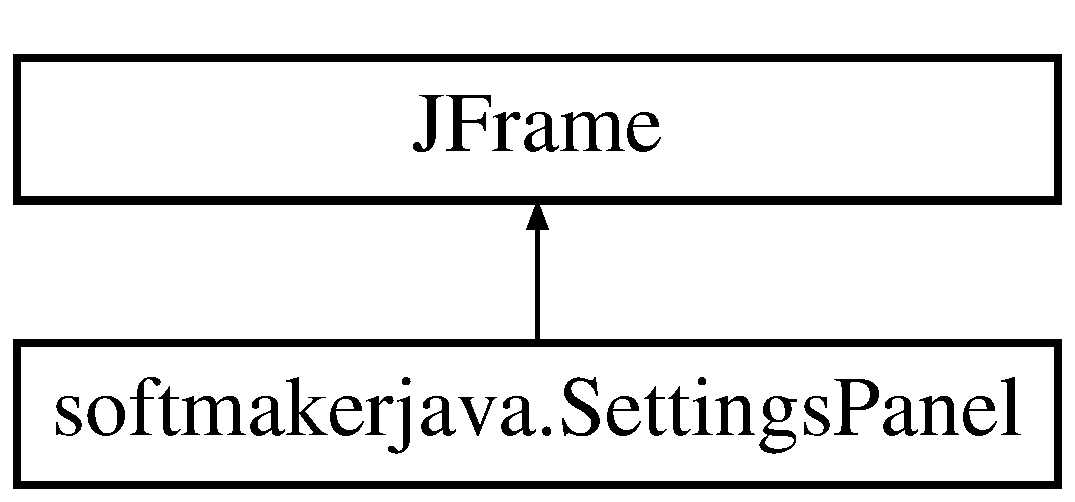
\includegraphics[height=2.000000cm]{classsoftmakerjava_1_1_settings_panel}
\end{center}
\end{figure}
\subsection*{Public Member Functions}
\begin{DoxyCompactItemize}
\item 
{\bfseries Settings\+Panel} (J\+Frame parent\+Frame)\hypertarget{classsoftmakerjava_1_1_settings_panel_acc09db6c0fbf482aa72d11f1832cc482}{}\label{classsoftmakerjava_1_1_settings_panel_acc09db6c0fbf482aa72d11f1832cc482}

\end{DoxyCompactItemize}
\subsection*{Private Member Functions}
\begin{DoxyCompactItemize}
\item 
void {\bfseries init\+Components} ()\hypertarget{classsoftmakerjava_1_1_settings_panel_a3fdde2a8e41a3a1fa866cdcd17ba1b02}{}\label{classsoftmakerjava_1_1_settings_panel_a3fdde2a8e41a3a1fa866cdcd17ba1b02}

\item 
void {\bfseries save\+But\+Action\+Performed} (java.\+awt.\+event.\+Action\+Event evt)\hypertarget{classsoftmakerjava_1_1_settings_panel_a605332892182ba820f9fba60252c115e}{}\label{classsoftmakerjava_1_1_settings_panel_a605332892182ba820f9fba60252c115e}

\item 
void {\bfseries cancel\+But\+Action\+Performed} (java.\+awt.\+event.\+Action\+Event evt)\hypertarget{classsoftmakerjava_1_1_settings_panel_ad9159a73ff79ff7dd2c7a56b45cf99b6}{}\label{classsoftmakerjava_1_1_settings_panel_ad9159a73ff79ff7dd2c7a56b45cf99b6}

\item 
void {\bfseries form\+Window\+Closing} (java.\+awt.\+event.\+Window\+Event evt)\hypertarget{classsoftmakerjava_1_1_settings_panel_ac4fe57308cf72295897e4fa2b6be46b8}{}\label{classsoftmakerjava_1_1_settings_panel_ac4fe57308cf72295897e4fa2b6be46b8}

\item 
void {\bfseries fill\+With\+Current\+Settings} ()\hypertarget{classsoftmakerjava_1_1_settings_panel_a485d2880274c5c7c0bb5bf6e829278b5}{}\label{classsoftmakerjava_1_1_settings_panel_a485d2880274c5c7c0bb5bf6e829278b5}

\end{DoxyCompactItemize}
\subsection*{Private Attributes}
\begin{DoxyCompactItemize}
\item 
final J\+Frame {\bfseries parent\+Frame}\hypertarget{classsoftmakerjava_1_1_settings_panel_a8ba5efeab5d2ce654e9f3cee0db83e25}{}\label{classsoftmakerjava_1_1_settings_panel_a8ba5efeab5d2ce654e9f3cee0db83e25}

\item 
javax.\+swing.\+J\+Label {\bfseries app\+Lan\+Label}\hypertarget{classsoftmakerjava_1_1_settings_panel_a164fa9ae3d12b3f5c08645211be70b65}{}\label{classsoftmakerjava_1_1_settings_panel_a164fa9ae3d12b3f5c08645211be70b65}

\item 
javax.\+swing.\+J\+Button {\bfseries cancel\+But}\hypertarget{classsoftmakerjava_1_1_settings_panel_a6449cb6e7ea6de65adb49370a8ce5e19}{}\label{classsoftmakerjava_1_1_settings_panel_a6449cb6e7ea6de65adb49370a8ce5e19}

\item 
javax.\+swing.\+J\+Combo\+Box {\bfseries code\+Combo}\hypertarget{classsoftmakerjava_1_1_settings_panel_a142819d7ae6868e15ccf688f6d030636}{}\label{classsoftmakerjava_1_1_settings_panel_a142819d7ae6868e15ccf688f6d030636}

\item 
javax.\+swing.\+J\+Label {\bfseries code\+Lan\+Label}\hypertarget{classsoftmakerjava_1_1_settings_panel_a19734e8ffe62900903975ad3a6f385ee}{}\label{classsoftmakerjava_1_1_settings_panel_a19734e8ffe62900903975ad3a6f385ee}

\item 
javax.\+swing.\+J\+Panel {\bfseries combo\+Panel}\hypertarget{classsoftmakerjava_1_1_settings_panel_a32b819c3be997032ebafff295339dbff}{}\label{classsoftmakerjava_1_1_settings_panel_a32b819c3be997032ebafff295339dbff}

\item 
javax.\+swing.\+J\+Text\+Field {\bfseries ip\+Field}\hypertarget{classsoftmakerjava_1_1_settings_panel_a16695b3df093b12d25809641f61869b7}{}\label{classsoftmakerjava_1_1_settings_panel_a16695b3df093b12d25809641f61869b7}

\item 
javax.\+swing.\+J\+Text\+Field {\bfseries port\+Field}\hypertarget{classsoftmakerjava_1_1_settings_panel_a11c61a8eee99d644af02d59f9bc29455}{}\label{classsoftmakerjava_1_1_settings_panel_a11c61a8eee99d644af02d59f9bc29455}

\item 
javax.\+swing.\+J\+Label {\bfseries s\+Ip\+Label}\hypertarget{classsoftmakerjava_1_1_settings_panel_a9d17ddd726cba4de0e3dd3cd21f488c9}{}\label{classsoftmakerjava_1_1_settings_panel_a9d17ddd726cba4de0e3dd3cd21f488c9}

\item 
javax.\+swing.\+J\+Label {\bfseries s\+Port\+Label}\hypertarget{classsoftmakerjava_1_1_settings_panel_a34e0c46ff07c9fcfa5fff302decd55e9}{}\label{classsoftmakerjava_1_1_settings_panel_a34e0c46ff07c9fcfa5fff302decd55e9}

\item 
javax.\+swing.\+J\+Button {\bfseries save\+But}\hypertarget{classsoftmakerjava_1_1_settings_panel_a52e188c20815bfd1e08610a615853aa3}{}\label{classsoftmakerjava_1_1_settings_panel_a52e188c20815bfd1e08610a615853aa3}

\item 
javax.\+swing.\+J\+Combo\+Box {\bfseries spoken\+Combo}\hypertarget{classsoftmakerjava_1_1_settings_panel_ad65ff8e0db0a961481fa8b15672073b7}{}\label{classsoftmakerjava_1_1_settings_panel_ad65ff8e0db0a961481fa8b15672073b7}

\end{DoxyCompactItemize}


\subsection{Detailed Description}
\begin{DoxyAuthor}{Author}
Baka 
\end{DoxyAuthor}


The documentation for this class was generated from the following file\+:\begin{DoxyCompactItemize}
\item 
C\+:/\+Users/\+Wojtek\+K/\+Desktop/\+Soft\+Maker\+Java1/src/softmakerjava/Settings\+Panel.\+java\end{DoxyCompactItemize}

\hypertarget{classsoftmakerjava_1_1_soft_maker_java}{}\section{softmakerjava.\+Soft\+Maker\+Java Class Reference}
\label{classsoftmakerjava_1_1_soft_maker_java}\index{softmakerjava.\+Soft\+Maker\+Java@{softmakerjava.\+Soft\+Maker\+Java}}
\subsection*{Static Public Member Functions}
\begin{DoxyCompactItemize}
\item 
static void \hyperlink{classsoftmakerjava_1_1_soft_maker_java_a4e5108a753f7a544bd78993b3f3028ae}{main} (String\mbox{[}$\,$\mbox{]} args)
\end{DoxyCompactItemize}


\subsection{Detailed Description}
\begin{DoxyAuthor}{Author}
Baka 
\end{DoxyAuthor}


\subsection{Member Function Documentation}
\index{softmakerjava\+::\+Soft\+Maker\+Java@{softmakerjava\+::\+Soft\+Maker\+Java}!main@{main}}
\index{main@{main}!softmakerjava\+::\+Soft\+Maker\+Java@{softmakerjava\+::\+Soft\+Maker\+Java}}
\subsubsection[{\texorpdfstring{main(\+String[] args)}{main(String[] args)}}]{\setlength{\rightskip}{0pt plus 5cm}static void softmakerjava.\+Soft\+Maker\+Java.\+main (
\begin{DoxyParamCaption}
\item[{String\mbox{[}$\,$\mbox{]}}]{args}
\end{DoxyParamCaption}
)\hspace{0.3cm}{\ttfamily [static]}}\hypertarget{classsoftmakerjava_1_1_soft_maker_java_a4e5108a753f7a544bd78993b3f3028ae}{}\label{classsoftmakerjava_1_1_soft_maker_java_a4e5108a753f7a544bd78993b3f3028ae}

\begin{DoxyParams}{Parameters}
{\em args} & the command line arguments \\
\hline
\end{DoxyParams}


The documentation for this class was generated from the following file\+:\begin{DoxyCompactItemize}
\item 
C\+:/\+Users/\+Wojtek\+K/\+Desktop/\+Soft\+Maker\+Java1/src/softmakerjava/Soft\+Maker\+Java.\+java\end{DoxyCompactItemize}

\hypertarget{classsoftmakerjava_1_1_task}{}\section{softmakerjava.\+Task Class Reference}
\label{classsoftmakerjava_1_1_task}\index{softmakerjava.\+Task@{softmakerjava.\+Task}}
\subsection*{Public Member Functions}
\begin{DoxyCompactItemize}
\item 
{\bfseries Task} (String name, Calendar deadline, String type)\hypertarget{classsoftmakerjava_1_1_task_adcd90fe2c7b6e296757c02cd7b93b355}{}\label{classsoftmakerjava_1_1_task_adcd90fe2c7b6e296757c02cd7b93b355}

\item 
void {\bfseries set\+Name} (String name)\hypertarget{classsoftmakerjava_1_1_task_a913f199ef73676529e6cd28cf3bc8cdb}{}\label{classsoftmakerjava_1_1_task_a913f199ef73676529e6cd28cf3bc8cdb}

\item 
String {\bfseries get\+Name} ()\hypertarget{classsoftmakerjava_1_1_task_aa88cc75b950a54e529bcc0a2086c0687}{}\label{classsoftmakerjava_1_1_task_aa88cc75b950a54e529bcc0a2086c0687}

\item 
Calendar {\bfseries get\+Deadline} ()\hypertarget{classsoftmakerjava_1_1_task_a935e974898f4d00b79bfc33b3f4dbc25}{}\label{classsoftmakerjava_1_1_task_a935e974898f4d00b79bfc33b3f4dbc25}

\item 
String {\bfseries get\+Type} ()\hypertarget{classsoftmakerjava_1_1_task_a5079c681e7f5f8b081c8e89276094bfa}{}\label{classsoftmakerjava_1_1_task_a5079c681e7f5f8b081c8e89276094bfa}

\item 
void {\bfseries set\+Deadline} (Calendar deadline)\hypertarget{classsoftmakerjava_1_1_task_a4171a9457ff8baa8c629a0fd5b4f4295}{}\label{classsoftmakerjava_1_1_task_a4171a9457ff8baa8c629a0fd5b4f4295}

\item 
void {\bfseries set\+Type} (String type)\hypertarget{classsoftmakerjava_1_1_task_a9575eff2b44c05df71b953112dd9b8c2}{}\label{classsoftmakerjava_1_1_task_a9575eff2b44c05df71b953112dd9b8c2}

\item 
void {\bfseries set\+Status} (String status)\hypertarget{classsoftmakerjava_1_1_task_a270d94ca0ed5bcc3d9c03fc2fcab7b1e}{}\label{classsoftmakerjava_1_1_task_a270d94ca0ed5bcc3d9c03fc2fcab7b1e}

\item 
String {\bfseries get\+Status} ()\hypertarget{classsoftmakerjava_1_1_task_ace5d3de273f4fa7d33f6890a6f6e98f9}{}\label{classsoftmakerjava_1_1_task_ace5d3de273f4fa7d33f6890a6f6e98f9}

\end{DoxyCompactItemize}
\subsection*{Private Attributes}
\begin{DoxyCompactItemize}
\item 
String {\bfseries name}\hypertarget{classsoftmakerjava_1_1_task_a55d0f97f41eb8b991acc7ec7a63744c8}{}\label{classsoftmakerjava_1_1_task_a55d0f97f41eb8b991acc7ec7a63744c8}

\item 
String {\bfseries type}\hypertarget{classsoftmakerjava_1_1_task_a8f23833bcc2220df044937de9fd04337}{}\label{classsoftmakerjava_1_1_task_a8f23833bcc2220df044937de9fd04337}

\item 
Calendar {\bfseries deadline}\hypertarget{classsoftmakerjava_1_1_task_a9bef5960037c78ba0a9b343843139231}{}\label{classsoftmakerjava_1_1_task_a9bef5960037c78ba0a9b343843139231}

\item 
String {\bfseries status}\hypertarget{classsoftmakerjava_1_1_task_af9414cf564efce8fa4cc15d1661e5d0d}{}\label{classsoftmakerjava_1_1_task_af9414cf564efce8fa4cc15d1661e5d0d}

\end{DoxyCompactItemize}


The documentation for this class was generated from the following file\+:\begin{DoxyCompactItemize}
\item 
C\+:/\+Users/\+Wojtek\+K/\+Desktop/\+Soft\+Maker\+Java1/src/softmakerjava/Task.\+java\end{DoxyCompactItemize}

\hypertarget{classsoftmakerjava_1_1_task_menager}{}\section{softmakerjava.\+Task\+Menager Class Reference}
\label{classsoftmakerjava_1_1_task_menager}\index{softmakerjava.\+Task\+Menager@{softmakerjava.\+Task\+Menager}}
\subsection*{Public Member Functions}
\begin{DoxyCompactItemize}
\item 
Vector$<$ \hyperlink{classsoftmakerjava_1_1_task}{Task} $>$ {\bfseries get\+Task\+Queue} ()\hypertarget{classsoftmakerjava_1_1_task_menager_ae25d4bb98fb417686a589501ed0121f5}{}\label{classsoftmakerjava_1_1_task_menager_ae25d4bb98fb417686a589501ed0121f5}

\item 
void {\bfseries set\+Task\+Queue} (\hyperlink{classsoftmakerjava_1_1_task}{Task} task\+Queue)\hypertarget{classsoftmakerjava_1_1_task_menager_a32477430eeeeb9702075b1255966e4f8}{}\label{classsoftmakerjava_1_1_task_menager_a32477430eeeeb9702075b1255966e4f8}

\item 
void {\bfseries Bind\+Task} (String username, String taskname)\hypertarget{classsoftmakerjava_1_1_task_menager_a6cb52154c2c806c19f37a75779ddc55e}{}\label{classsoftmakerjava_1_1_task_menager_a6cb52154c2c806c19f37a75779ddc55e}

\item 
void {\bfseries Add\+New\+Task} (\hyperlink{classsoftmakerjava_1_1_task}{Task} task)\hypertarget{classsoftmakerjava_1_1_task_menager_aa095af57950e2420097b7445ac635a9b}{}\label{classsoftmakerjava_1_1_task_menager_aa095af57950e2420097b7445ac635a9b}

\item 
void {\bfseries Remove\+Task} (\hyperlink{classsoftmakerjava_1_1_task}{Task} task)\hypertarget{classsoftmakerjava_1_1_task_menager_a9d541a154cfc02fd10ab6c0ec53ba14e}{}\label{classsoftmakerjava_1_1_task_menager_a9d541a154cfc02fd10ab6c0ec53ba14e}

\item 
boolean {\bfseries Validate\+Task} (\hyperlink{classsoftmakerjava_1_1_task}{Task} task)\hypertarget{classsoftmakerjava_1_1_task_menager_af79e2d99c4d18d639fd243f904e9065f}{}\label{classsoftmakerjava_1_1_task_menager_af79e2d99c4d18d639fd243f904e9065f}

\item 
Vector {\bfseries Generate\+Task\+List} ()\hypertarget{classsoftmakerjava_1_1_task_menager_ae2df7d0a47145218a73d03974883cfb9}{}\label{classsoftmakerjava_1_1_task_menager_ae2df7d0a47145218a73d03974883cfb9}

\end{DoxyCompactItemize}
\subsection*{Private Attributes}
\begin{DoxyCompactItemize}
\item 
Vector$<$ \hyperlink{classsoftmakerjava_1_1_task}{Task} $>$ {\bfseries task\+Queue} = new Vector$<$\hyperlink{classsoftmakerjava_1_1_task}{Task}$>$(1)\hypertarget{classsoftmakerjava_1_1_task_menager_aa7c89025a8d1118ff5159061fb4f2a90}{}\label{classsoftmakerjava_1_1_task_menager_aa7c89025a8d1118ff5159061fb4f2a90}

\end{DoxyCompactItemize}


The documentation for this class was generated from the following file\+:\begin{DoxyCompactItemize}
\item 
C\+:/\+Users/\+Wojtek\+K/\+Desktop/\+Soft\+Maker\+Java1/src/softmakerjava/Task\+Menager.\+java\end{DoxyCompactItemize}

\hypertarget{classsoftmakerjava_1_1_task_panel}{}\section{softmakerjava.\+Task\+Panel Class Reference}
\label{classsoftmakerjava_1_1_task_panel}\index{softmakerjava.\+Task\+Panel@{softmakerjava.\+Task\+Panel}}
Inheritance diagram for softmakerjava.\+Task\+Panel\+:\begin{figure}[H]
\begin{center}
\leavevmode
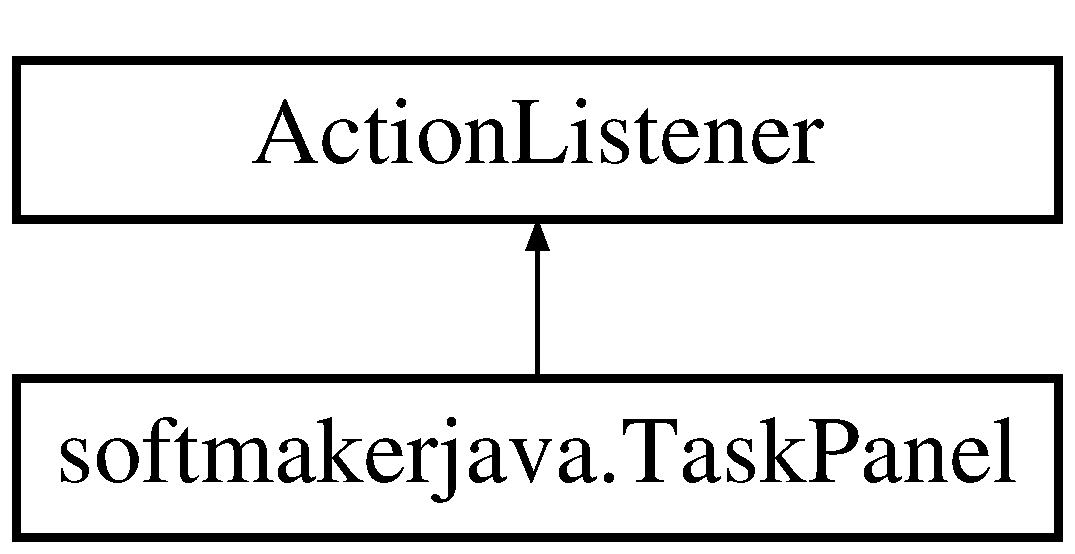
\includegraphics[height=2.000000cm]{classsoftmakerjava_1_1_task_panel}
\end{center}
\end{figure}
\subsection*{Public Member Functions}
\begin{DoxyCompactItemize}
\item 
void {\bfseries action\+Performed} (Action\+Event e)\hypertarget{classsoftmakerjava_1_1_task_panel_aec564204f53ff71f7d8f347a5e06287c}{}\label{classsoftmakerjava_1_1_task_panel_aec564204f53ff71f7d8f347a5e06287c}

\end{DoxyCompactItemize}
\subsection*{Private Member Functions}
\begin{DoxyCompactItemize}
\item 
void {\bfseries prepare\+G\+UI} ()\hypertarget{classsoftmakerjava_1_1_task_panel_a8c018ddc0ca0cb57df9cd0313fc97ded}{}\label{classsoftmakerjava_1_1_task_panel_a8c018ddc0ca0cb57df9cd0313fc97ded}

\item 
void {\bfseries filter\+Tasks} ()\hypertarget{classsoftmakerjava_1_1_task_panel_a03f6f39278caf4269caf457b7e6dc072}{}\label{classsoftmakerjava_1_1_task_panel_a03f6f39278caf4269caf457b7e6dc072}

\item 
void {\bfseries group\+Tasks} ()\hypertarget{classsoftmakerjava_1_1_task_panel_a02c79a5bbb164db796f15ab08cdd1f63}{}\label{classsoftmakerjava_1_1_task_panel_a02c79a5bbb164db796f15ab08cdd1f63}

\end{DoxyCompactItemize}
\subsection*{Private Attributes}
\begin{DoxyCompactItemize}
\item 
J\+Frame {\bfseries main\+Frame}\hypertarget{classsoftmakerjava_1_1_task_panel_ae59a80e7dc11390635d917ccb9a3fcb5}{}\label{classsoftmakerjava_1_1_task_panel_ae59a80e7dc11390635d917ccb9a3fcb5}

\item 
J\+Label {\bfseries UserL}\hypertarget{classsoftmakerjava_1_1_task_panel_a6f845d2193d9c4a32912952ee704c120}{}\label{classsoftmakerjava_1_1_task_panel_a6f845d2193d9c4a32912952ee704c120}

\item 
J\+Combo\+Box {\bfseries Users}\hypertarget{classsoftmakerjava_1_1_task_panel_a9f6993a1b22d9ee357db6503bf75f052}{}\label{classsoftmakerjava_1_1_task_panel_a9f6993a1b22d9ee357db6503bf75f052}

\item 
J\+Combo\+Box {\bfseries Tasks}\hypertarget{classsoftmakerjava_1_1_task_panel_ab5e0554a47a76e24e71942e757ec46f9}{}\label{classsoftmakerjava_1_1_task_panel_ab5e0554a47a76e24e71942e757ec46f9}

\item 
J\+Button {\bfseries Bind\+Task}\hypertarget{classsoftmakerjava_1_1_task_panel_ac3b5013c15cfe518a4595488deb6c839}{}\label{classsoftmakerjava_1_1_task_panel_ac3b5013c15cfe518a4595488deb6c839}

\item 
J\+Text\+Field {\bfseries Name}\hypertarget{classsoftmakerjava_1_1_task_panel_ad7a8886a63dcf3c7c0aeed5cbe4f9204}{}\label{classsoftmakerjava_1_1_task_panel_ad7a8886a63dcf3c7c0aeed5cbe4f9204}

\item 
J\+Text\+Field {\bfseries Type}\hypertarget{classsoftmakerjava_1_1_task_panel_aeb2fa1b1ba468dc5e679b2eafbcbd5a2}{}\label{classsoftmakerjava_1_1_task_panel_aeb2fa1b1ba468dc5e679b2eafbcbd5a2}

\item 
J\+Text\+Field {\bfseries Deadline}\hypertarget{classsoftmakerjava_1_1_task_panel_a300ed8119c6f54489d1af539edcd168c}{}\label{classsoftmakerjava_1_1_task_panel_a300ed8119c6f54489d1af539edcd168c}

\item 
J\+Button {\bfseries Add\+Task}\hypertarget{classsoftmakerjava_1_1_task_panel_aef3057f67a6d21ed05df83a1625164b1}{}\label{classsoftmakerjava_1_1_task_panel_aef3057f67a6d21ed05df83a1625164b1}

\item 
J\+Combo\+Box {\bfseries Tasks\+Del}\hypertarget{classsoftmakerjava_1_1_task_panel_a8fd8c0aeb47bb0ebd42642e4a706de0b}{}\label{classsoftmakerjava_1_1_task_panel_a8fd8c0aeb47bb0ebd42642e4a706de0b}

\item 
J\+Button {\bfseries Del\+Btn}\hypertarget{classsoftmakerjava_1_1_task_panel_adbc49df13545eff13216238fe2f90689}{}\label{classsoftmakerjava_1_1_task_panel_adbc49df13545eff13216238fe2f90689}

\item 
J\+Combo\+Box {\bfseries Tasks\+Val}\hypertarget{classsoftmakerjava_1_1_task_panel_ab1d62a5c0cfb1e893085c79aaa9a54db}{}\label{classsoftmakerjava_1_1_task_panel_ab1d62a5c0cfb1e893085c79aaa9a54db}

\item 
J\+Button {\bfseries Val\+Btn}\hypertarget{classsoftmakerjava_1_1_task_panel_a1453a3fbe8d79b0df25addb328801be7}{}\label{classsoftmakerjava_1_1_task_panel_a1453a3fbe8d79b0df25addb328801be7}

\item 
J\+Button {\bfseries Generate\+Btn}\hypertarget{classsoftmakerjava_1_1_task_panel_a4859bcfabeffa09693f6a2c146e53f9f}{}\label{classsoftmakerjava_1_1_task_panel_a4859bcfabeffa09693f6a2c146e53f9f}

\item 
J\+Button {\bfseries Close\+Btn}\hypertarget{classsoftmakerjava_1_1_task_panel_ac77b3d07f600eb64ea912b61cd27906b}{}\label{classsoftmakerjava_1_1_task_panel_ac77b3d07f600eb64ea912b61cd27906b}

\item 
J\+Text\+Field {\bfseries U\+Name}\hypertarget{classsoftmakerjava_1_1_task_panel_a2d459c0b115f88c39c88e31284681ced}{}\label{classsoftmakerjava_1_1_task_panel_a2d459c0b115f88c39c88e31284681ced}

\item 
J\+Button {\bfseries U\+Add}\hypertarget{classsoftmakerjava_1_1_task_panel_a6f4d94c144330364d54f3a2155224ad9}{}\label{classsoftmakerjava_1_1_task_panel_a6f4d94c144330364d54f3a2155224ad9}

\end{DoxyCompactItemize}


The documentation for this class was generated from the following file\+:\begin{DoxyCompactItemize}
\item 
C\+:/\+Users/\+Wojtek\+K/\+Desktop/\+Soft\+Maker\+Java1/src/softmakerjava/Task\+Panel.\+java\end{DoxyCompactItemize}

\hypertarget{classsoftmakerjava_1_1_user}{}\section{softmakerjava.\+User Class Reference}
\label{classsoftmakerjava_1_1_user}\index{softmakerjava.\+User@{softmakerjava.\+User}}
\subsection*{Public Member Functions}
\begin{DoxyCompactItemize}
\item 
{\bfseries User} (String name, String status, String position)\hypertarget{classsoftmakerjava_1_1_user_a6329a37981910cec226ce23aad8bfdcc}{}\label{classsoftmakerjava_1_1_user_a6329a37981910cec226ce23aad8bfdcc}

\item 
String {\bfseries get\+Name} ()\hypertarget{classsoftmakerjava_1_1_user_a33dcaf750bd4b95f6da89e773cb9ee8e}{}\label{classsoftmakerjava_1_1_user_a33dcaf750bd4b95f6da89e773cb9ee8e}

\item 
String {\bfseries get\+Position} ()\hypertarget{classsoftmakerjava_1_1_user_ad6bbbfa19a77534f020bf7646bcbeae7}{}\label{classsoftmakerjava_1_1_user_ad6bbbfa19a77534f020bf7646bcbeae7}

\item 
String {\bfseries get\+Status} ()\hypertarget{classsoftmakerjava_1_1_user_a1763522c917bedcb5c07221e3a07ff71}{}\label{classsoftmakerjava_1_1_user_a1763522c917bedcb5c07221e3a07ff71}

\item 
Vector {\bfseries get\+Tasks} ()\hypertarget{classsoftmakerjava_1_1_user_acc5945d8b6c5e3517d96019ccf2fe605}{}\label{classsoftmakerjava_1_1_user_acc5945d8b6c5e3517d96019ccf2fe605}

\item 
int {\bfseries getid} ()\hypertarget{classsoftmakerjava_1_1_user_af783a3e6819199ff4d238126462a6f25}{}\label{classsoftmakerjava_1_1_user_af783a3e6819199ff4d238126462a6f25}

\item 
void {\bfseries set\+Id} (int id)\hypertarget{classsoftmakerjava_1_1_user_a9378481c26f2b0010ea3ef7c11d6c402}{}\label{classsoftmakerjava_1_1_user_a9378481c26f2b0010ea3ef7c11d6c402}

\item 
void {\bfseries set\+Name} (String name)\hypertarget{classsoftmakerjava_1_1_user_a8b082d25d2ca7e051eb993efa51e2c87}{}\label{classsoftmakerjava_1_1_user_a8b082d25d2ca7e051eb993efa51e2c87}

\item 
void {\bfseries set\+Position} (String position)\hypertarget{classsoftmakerjava_1_1_user_ad29eab622ffef70d52305b7351db28ce}{}\label{classsoftmakerjava_1_1_user_ad29eab622ffef70d52305b7351db28ce}

\item 
void {\bfseries set\+Status} (String status)\hypertarget{classsoftmakerjava_1_1_user_a95c4fa67e8714f0a444c837c3d6f4cd4}{}\label{classsoftmakerjava_1_1_user_a95c4fa67e8714f0a444c837c3d6f4cd4}

\item 
void {\bfseries set\+Task} (\hyperlink{classsoftmakerjava_1_1_task}{Task} task)\hypertarget{classsoftmakerjava_1_1_user_a9c5b2a2f11a37caeff61e462506c1728}{}\label{classsoftmakerjava_1_1_user_a9c5b2a2f11a37caeff61e462506c1728}

\end{DoxyCompactItemize}
\subsection*{Private Attributes}
\begin{DoxyCompactItemize}
\item 
int {\bfseries id}\hypertarget{classsoftmakerjava_1_1_user_a4ce23be841fd125ad6629a5fe2102466}{}\label{classsoftmakerjava_1_1_user_a4ce23be841fd125ad6629a5fe2102466}

\item 
String {\bfseries name}\hypertarget{classsoftmakerjava_1_1_user_ad6ffdb13839bffb212c60a5e8dd29efd}{}\label{classsoftmakerjava_1_1_user_ad6ffdb13839bffb212c60a5e8dd29efd}

\item 
String {\bfseries status}\hypertarget{classsoftmakerjava_1_1_user_a1e1c95a7f54b640c72cbe2dc3b83d182}{}\label{classsoftmakerjava_1_1_user_a1e1c95a7f54b640c72cbe2dc3b83d182}

\item 
String {\bfseries position}\hypertarget{classsoftmakerjava_1_1_user_a56188006e7443054457de5617d6dba62}{}\label{classsoftmakerjava_1_1_user_a56188006e7443054457de5617d6dba62}

\end{DoxyCompactItemize}


The documentation for this class was generated from the following file\+:\begin{DoxyCompactItemize}
\item 
C\+:/\+Users/\+Wojtek\+K/\+Desktop/\+Soft\+Maker\+Java1/src/softmakerjava/User.\+java\end{DoxyCompactItemize}

\hypertarget{classsoftmakerjava_1_1_user_center}{}\section{softmakerjava.\+User\+Center Class Reference}
\label{classsoftmakerjava_1_1_user_center}\index{softmakerjava.\+User\+Center@{softmakerjava.\+User\+Center}}
\subsection*{Public Member Functions}
\begin{DoxyCompactItemize}
\item 
Vector$<$ \hyperlink{classsoftmakerjava_1_1_task}{Task} $>$ {\bfseries Show\+User\+Tasks} (\hyperlink{classsoftmakerjava_1_1_user}{User} current\+User)\hypertarget{classsoftmakerjava_1_1_user_center_a4fd011aae2210dc1b39397590e7134c9}{}\label{classsoftmakerjava_1_1_user_center_a4fd011aae2210dc1b39397590e7134c9}

\item 
void {\bfseries Deploy\+Task} (String Task\+Name)\hypertarget{classsoftmakerjava_1_1_user_center_a661950f4f0e212a003a4a37ee0363d30}{}\label{classsoftmakerjava_1_1_user_center_a661950f4f0e212a003a4a37ee0363d30}

\end{DoxyCompactItemize}


The documentation for this class was generated from the following file\+:\begin{DoxyCompactItemize}
\item 
C\+:/\+Users/\+Wojtek\+K/\+Desktop/\+Soft\+Maker\+Java1/src/softmakerjava/User\+Center.\+java\end{DoxyCompactItemize}

\hypertarget{classsoftmakerjava_1_1_user_repository}{}\section{softmakerjava.\+User\+Repository Class Reference}
\label{classsoftmakerjava_1_1_user_repository}\index{softmakerjava.\+User\+Repository@{softmakerjava.\+User\+Repository}}
\subsection*{Public Member Functions}
\begin{DoxyCompactItemize}
\item 
void {\bfseries Load\+User} ()\hypertarget{classsoftmakerjava_1_1_user_repository_a8af4cd8b22e04fb4daa66d2533e2ed7e}{}\label{classsoftmakerjava_1_1_user_repository_a8af4cd8b22e04fb4daa66d2533e2ed7e}

\item 
void {\bfseries Add\+User} (String name, String status, String position)\hypertarget{classsoftmakerjava_1_1_user_repository_aac2ef6e3d85131bab140abbcda29e4e2}{}\label{classsoftmakerjava_1_1_user_repository_aac2ef6e3d85131bab140abbcda29e4e2}

\item 
void {\bfseries Delete\+User} (String Name)\hypertarget{classsoftmakerjava_1_1_user_repository_a611f357a1bb5cf6b2cf49aab36452c61}{}\label{classsoftmakerjava_1_1_user_repository_a611f357a1bb5cf6b2cf49aab36452c61}

\item 
void {\bfseries Load\+Online\+Users} ()\hypertarget{classsoftmakerjava_1_1_user_repository_a79745f400ee62bb6adf9cf2901dfdedd}{}\label{classsoftmakerjava_1_1_user_repository_a79745f400ee62bb6adf9cf2901dfdedd}

\end{DoxyCompactItemize}
\subsection*{Static Public Member Functions}
\begin{DoxyCompactItemize}
\item 
static void {\bfseries main} (String\mbox{[}$\,$\mbox{]} args)\hypertarget{classsoftmakerjava_1_1_user_repository_a656cd4f239337a13475d244acc1cacca}{}\label{classsoftmakerjava_1_1_user_repository_a656cd4f239337a13475d244acc1cacca}

\end{DoxyCompactItemize}
\subsection*{Public Attributes}
\begin{DoxyCompactItemize}
\item 
Vector$<$ \hyperlink{classsoftmakerjava_1_1_user}{User} $>$ {\bfseries users} = new Vector(0)\hypertarget{classsoftmakerjava_1_1_user_repository_a02b286c04b3cebe586ad9de198669d0b}{}\label{classsoftmakerjava_1_1_user_repository_a02b286c04b3cebe586ad9de198669d0b}

\end{DoxyCompactItemize}


The documentation for this class was generated from the following file\+:\begin{DoxyCompactItemize}
\item 
C\+:/\+Users/\+Wojtek\+K/\+Desktop/\+Soft\+Maker\+Java1/src/softmakerjava/User\+Repository.\+java\end{DoxyCompactItemize}

\hypertarget{classsoftmakerjava_1_1_validator}{}\section{softmakerjava.\+Validator Class Reference}
\label{classsoftmakerjava_1_1_validator}\index{softmakerjava.\+Validator@{softmakerjava.\+Validator}}
\subsection*{Public Member Functions}
\begin{DoxyCompactItemize}
\item 
boolean {\bfseries Check\+Validation} (\hyperlink{classsoftmakerjava_1_1_task}{Task} task)\hypertarget{classsoftmakerjava_1_1_validator_ac3d368de65875241e7c6636dca24627d}{}\label{classsoftmakerjava_1_1_validator_ac3d368de65875241e7c6636dca24627d}

\item 
void {\bfseries Mark\+Task\+As\+Completed} (\hyperlink{classsoftmakerjava_1_1_task}{Task} task)\hypertarget{classsoftmakerjava_1_1_validator_a7c363b5e2d71a53e81a52c459580f53c}{}\label{classsoftmakerjava_1_1_validator_a7c363b5e2d71a53e81a52c459580f53c}

\item 
void {\bfseries Mark\+Task\+As\+Failed} (\hyperlink{classsoftmakerjava_1_1_task}{Task} task)\hypertarget{classsoftmakerjava_1_1_validator_a012e45c2a22e305c248e1722ab7cb30b}{}\label{classsoftmakerjava_1_1_validator_a012e45c2a22e305c248e1722ab7cb30b}

\end{DoxyCompactItemize}
\subsection*{Private Member Functions}
\begin{DoxyCompactItemize}
\item 
boolean {\bfseries Get\+Test\+Results} (\hyperlink{classsoftmakerjava_1_1_task}{Task} task)\hypertarget{classsoftmakerjava_1_1_validator_a7676a8cf6cc9d5673704a2512ab03cc6}{}\label{classsoftmakerjava_1_1_validator_a7676a8cf6cc9d5673704a2512ab03cc6}

\item 
boolean {\bfseries Get\+Stats} (\hyperlink{classsoftmakerjava_1_1_task}{Task} task)\hypertarget{classsoftmakerjava_1_1_validator_a0f668559db973289cec25aa153eed2c9}{}\label{classsoftmakerjava_1_1_validator_a0f668559db973289cec25aa153eed2c9}

\end{DoxyCompactItemize}


The documentation for this class was generated from the following file\+:\begin{DoxyCompactItemize}
\item 
C\+:/\+Users/\+Wojtek\+K/\+Desktop/\+Soft\+Maker\+Java1/src/softmakerjava/Validator.\+java\end{DoxyCompactItemize}

%--- End generated contents ---

% Index
\backmatter
\newpage
\phantomsection
\clearemptydoublepage
\addcontentsline{toc}{chapter}{Index}
\printindex

\end{document}
